Este capítulo apresenta as principais definições e conceitos relacionados com a Computação em Nuvem, tais como: as características essenciais, os tipos de serviço, os tipos de implantação e alguns conceitos e ferramentas importantes para a funcionamento da nuvem.


A Computação em Nuvem (\textit{Cloud Computing}) é uma tecnologia que permite oferecer acesso remoto a software e executar diversas tarefas utilizando a Internet. Ela representa a infraestrutura de comunicação entre os componentes arquiteturais, baseada em uma abstração que oculta à complexidade de infraestrutura. Cada parte desta infraestrutura é provida como um serviço utilizando hardware compartilhado para computação e armazenamento.
Neste capítulo, serão definidas as características essenciais, os tipos de serviço, os tipos de implantação e uma definição resumida dos principais conceitos e ferramentas utilizadas na Computação em Nuvem \cite{ERCEMAPI2009}. 

\begin{quote}
\textit{"O modelo de computação em nuvem foi desenvolvido com o objetivo de fornecer serviços de fácil acesso, baixo custo e com garantias de disponibilidade e escalabilidade. Este modelo visa fornecer, basicamente, três benefícios. O primeiro benefício é reduzir o custo na aquisição e composição de toda infraestrutura requerida para atender as necessidades das empresas, podendo essa infraestrutura ser composta sob demanda e com recursos heterogêneos e de menor custo. O segundo é a flexibilidade que esse modelo oferece no que diz respeito à adição e substituição de recursos computacionais, podendo escalar tanto em nível de recursos de hardware quanto software para atender as necessidades das empresas e usuários. O último benefício é prover uma abstração e facilidade de acesso aos usuários destes serviços. Neste sentido, os usuários dos serviços não precisam conhecer aspectos de localização física e de entrega dos resultados destes serviços"} \cite{ERCEMAPI2009}.
\end{quote}

\section{Características Essenciais}

Pode-se definir e diferenciar a Computação em Nuvem de outros paradigmas quando combina-se algumas de suas características. Por exemplo, a elasticidade rápida de recursos, amplo acesso e a medição de serviço são características essenciais para compor uma solução de Computação em Nuvem \cite{ERCEMAPI2009}.

As características essenciais da Computação em Nuvem são:

\begin{itemize}
  \item Requisição de serviço sob demanda: o usuário pode adquirir unilateralmente recurso computacional na medida em que necessite e sem precisar de interação humana com os provedores de cada serviço, como tempo de procesamento no servidor ou armazenamento na rede. A infraestrutura dentro de uma nuvem podem ser automaticamente reconfigurada e/ou modificada e estas ações são transparentes para os usuários \cite{ERCEMAPI2009}.
  
  \item Amplo acesso: recursos são disponibilizados via Internet e acessados por meio de mecanismos padronizados que possibilitam o uso com plataformas \textit{thin}, tais como celulares, \textit{laptops} e PDAs. A interface de acesso à nuvem não obriga os usuários a mudar suas condições e ambientes de trabalho, como por exemplo, linguagens de programação e sistema operacional \cite{ERCEMAPI2009}.
  
  \item Portifólio de Recursos: os recursos computacionais do provedor são disponibilizados para servir múltiplos usuários usando um modelo \textit{multi-tenant} ou multi-inquilino, com diferentes recursos físicos e virtuais, dinamicamente atribuídos e ajustados de acordo com a demanda dos usuários. Estes usuários não precisam ter conhecimento da localização física dos recursos computacionais, podendo somente especificar a localização em um nível mais alto de abstração, tais como o país, estado ou centro de dados \cite{ERCEMAPI2009}.
  
  \item Elasticidade Rápida: recursos podem ser adquiridos de forma rápida e elástica. Em alguns casos automaticamente, se houver a necessidade de aumentar a quantidade disponibilizada de recursos, dado o aumento da demanda. Além disso, pode ser realocado quando há retração dessa demanda. Para os usuários, os recursos disponíveis parecem ser ilimitados e podem ser adquiridos em qualquer quantidade e a qualquer momento. A virtualização auxilia a elasticidade rápida ao criar várias instâncias de recursos requisitados utilizando um único recurso real. É através da virtualização que se pode abstrair características físicas de uma plataforma computacional dos usuários, exibindo outro hardware virtual e emulando um ou mais ambientes que podem ser independentes ou não \cite{ERCEMAPI2009}.
  
  \item Serviço Medido: sistemas em nuvem controlam e otimizam, automaticamente, o uso de recursos por meio de uma capacidade de medição. A automação é realizada em algum nível de abstração apropriado para o tipo de serviço, tais como armazenamento, processamento, largura de banda e contas dos usuários ativos. O uso de recursos pode ser monitorado e controlado, possibilitando transparência para o provedor e o usuário do serviço utilizado. Para garantir a qualidade do serviço, ou \textit{Quality of Service} (QoS), pode-se utilizar a abordagem baseada em acordo de nível de serviço, ou \textit{Services Level Agreement} (SLA). O SLA fornece informações sobre os níveis de disponibilidade, funcionalidade, desempenho e pode até mesmo estabelecer penalidades em caso de violação destes níveis \cite{ERCEMAPI2009}.
  
\end{itemize}

\section{Tipos de Serviço}
De acordo com \cite{JISA2010}, o modelo de negócios orientado a serviços é dividido em:

\begin{itemize}
  \item Software como Serviço (Saas): a aplicação é disponibilizada via Internet para que o cliente utilize conforme sua necessidade;
  \item Plataforma como Serviço (Paas): oferece partes de um ambiente ou de um sistema operacional completo, de forma que os usuários possam acessá-los remotamente;
  \item Infraestrutura como serviço (Iaas): objetivo é oferecer a infraestrutura de hardware de forma remota e transparente.
\end{itemize}

A Figura \ref{fig:modelo-servicos} exibe os tipos de serviços oferecidos na Computação em Nuvem e os relacionamentos entre eles.

\begin{figure}[H]
\centering
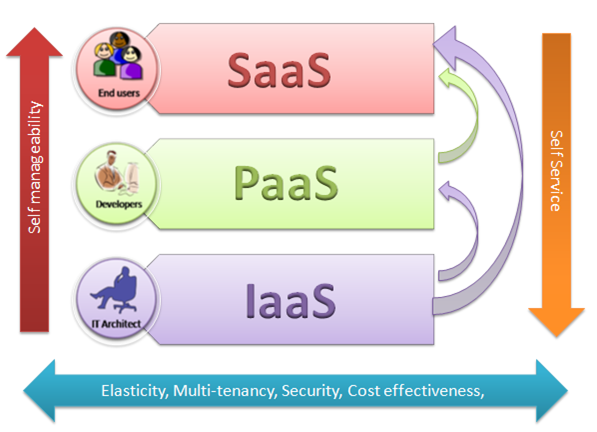
\includegraphics[scale=1]{imagens/delivery_models.png}
\caption{Modelos de Serviços em Computação em Nuvem}\cite{Alhamad2010}
\label{fig:modelo-servicos}
\end{figure}

\section{Tipos de implantação}
Pode-se classificar a estrutura disponível para os ambientes de computação em nuvem, em quatro diferentes tipos:

\begin{itemize}
  \item Público: Uma nuvem em que os prestadores de serviços oferecem seus recursos como serviços para o público em geral. As nuvens públicas oferecem vários benefícios importantes, incluindo nenhum investimento inicial em infraestrutura e deslocamento dos riscos para os fornecedores de infraestrutura. No entanto, a falta de controle refinado sobre as definições de dados, rede e segurança dificulta a eficácia em muitos cenários de negócios \cite{JISA2010}.
  
  \item Privado:  Também conhecido como nuvens internas, as nuvens privadas são projetadas para uso exclusivo por uma única organização. Uma nuvem privada pode ser construída e gerida pela organização ou por provedores externos. Esta oferece o mais alto grau de controle sobre o desempenho, confiabilidade e segurança. No entanto, são semelhantes à servidores proprietários tradicionais e não oferecem benefícios como redução nos custos de capital inicial \cite{JISA2010}.
  
  \item Híbrido: Uma nuvem híbrida é uma combinação de modelos de nuvens públicas e privadas, que tenta resolver as limitações de cada abordagem. Em uma nuvem híbrida, parte da infra-estrutura de serviço é executado em nuvens privadas, enquanto os demais serviços são executados em nuvens públicas. Nuvens híbridas são mais flexíveis que as nuvens públicas e privadas. Especificamente, estas proveem maior controle e segurança sobre os dados de aplicativos em comparação com as nuvens públicas, ao mesmo tempo facilitando a expansão dos serviços e contração de mais recursos. Projetar uma nuvem híbrida requer determinar cuidadosamente a melhor separação entre os componentes de nuvem pública e privada \cite{JISA2010}.
  
  \item Nuvem Privada Virtual: Uma solução alternativa para enfrentar as limitações de nuvens públicas e privadas é chamada como Nuvem Privada Virtual (\textit{Virtual Private Cloud} (VPC)). A VPC é essencialmente uma plataforma executada sobre nuvens públicas, sendo que a principal diferença é que esta aproveita a tecnologia de Rede Privada Virtual (VPN). O que permite aos provedores de serviços projetar suas próprias configurações de topologia e segurança, tais como regras de \textit{firewall}. VPC é essencialmente um projeto mais abrangente, uma vez que não só virtualiza servidores e aplicações, mas também a rede de comunicação subjacente. Além disso, para a maioria das empresas, VPC fornece transição suave de uma infra-estrutura de serviço proprietária para uma infra-estrutura baseada em nuvem pública, devido à camada de rede virtualizada \cite{JISA2010}.
  
\end{itemize}

\section{Conceitos e Ferramentas Importantes}

Nos ambientes de computação em nuvem, são utilizadas estruturas para suportar a escalabilidade, portabilidade, paralelismo e sincronismo de dados. Os termos e ferramentas citados a seguir compõe grande parte dos ambientes em nuvem. 

\begin{itemize}
  \item \textit{Hadoop}: É um projeto de software livre desenvolvido pela Apache Software Foundation, que é uma plataforma de computação distribuída, com alta escalabilidade, grande confiabilidade e tolerância a falhas.
  A biblioteca \textit{Hadoop} é um \textit{framework} que permite o processamento distribuído de grandes conjuntos de dados através de \textit{clusters} de computadores usando modelos de programação simples. Ele é projetado para garantir larga escalabilidade partindo de um único servidor até um \textit{cluster} com milhares de máquinas, sendo que cada máquina oferece capacidade de computação e armazenamento local. Ao invés de confiar no hardware para proporcionar maior disponibilidade, a própria biblioteca foi projetada para detectar e tratar falhas na camada de aplicação, de modo a fornecer um serviço com alta disponibilidade baseado em uma grade de computadores \cite{hadoop}. Um exemplo de utilização do \textit{Hadoop} é a técnica \textit{MapReduce}.
    \item \textit{MapReduce}: é uma técnica de processamento introduzida pela Google para suportar um grande conjunto de dados por meio de computação distribuída. Nela os dados são divididos através da função \textit{Map}, para que o processamento dos dados sejam feitos em paralelo. Logo após, é aplicada a função de \textit{Reduce} que consolida os dados processados e o retorna ao solicitante \cite{mapreduce}.
  \item \textit{Host}: é a máquina física que fornece os recursos de computação, como: memória, capacidade de processamento, armazenamento em disco, rede de I/O, entre outros. Estes recursos são utilizados pelos sistemas operacionais e demais ferramentas necessárias para virtualização \cite{Technology}.
  \item Virtualização: A virtualização é uma tecnologia que oferece uma camada de abstração dos verdadeiros recursos de uma máquina, provendo um hardware virtual para cada sistema. O objetivo é mascarar as características físicas e a forma como os sistemas operacionais e aplicações interagem com os recursos computacionais.
  
  \item \textit{Guest}: neste trabalho, o termo \textit{guest} é tratado como sinônimo de máquina virtual, que é um espaço virtual isolado com acesso ao hardware, onde funciona um sistema virtual. A utilização de \textit{guests} permite que diferentes aplicações, de diferentes plataformas, executem ao mesmo tempo em um mesmo hardware. Desta forma, as principais qualidades da virtualização são: o reaproveitamento de recursos, a portabilidade e a segurança; itens estes essenciais para a computação em nuvem \cite{ERCEMAPI2009}.
  \item KVM: \textit{Kernel-based Virtual Machine} é um módulo que provê a pilha de \textit{software} necessária para virtualização \cite{kvm}. Ele é um \textit{software} de código aberto que permite a criação de \textit{guests} e também é visto como um subsistema do Linux, uma vez que seu componente de \textit{kernel} está incluído nas distribuições Linux (a partir da versão 2.6.20
\end{itemize}